% !TEX root = ../CedricDe Schepper2023_Thesis.tex

\section{Results / Evaluation}\label{sec:results}

In order to evaluate the results from the analyses, we have to verify whether the phases perform their objective as described. First, does the initialisation phase succeed in generating a feasible solution, namely one without or with a minimal number of hard constraint violations? Second, does the optimisation phase succeed in significantly improving the exam distribution?

\subsection{Reference solutions}

The actual exam schedules, manually created by the administration of the University of Antwerp, can be used as a baseline to compare the generated schedules. These exam distributions can be seen in Figures \ref{fig:manual_sem1} and \ref{fig:manual_sem2}. Figure \ref{fig:manual_combined} shows the exam distribution when combining the schedule of both the Faculty of Applied engineering and the Faculty of  Science. Most notably, the manual schedules have a focus on keeping the amount of same day exams to a minimum and having 2 or more days in between exams as much as possible. This distribution is especially visible in the schedules for the Faculty of Applied Engineering. In order to be considered a superior solution, automatically generated schedules will have to minimise the amount of exams with fewer than 2 days in between, with a focus on same day exam violations.

Some additional observations can be made. First, it can be seen that the schedule for the faculty of Science contains a high amount of exam conflicts. Second, the exam distribution is much worse for the January exam period compared to that of June. This can clearly be seen in the combined exam distribution shown in Table \ref{fig:manual_combined}. This can be mostly be explained by January having more exams within a smaller period. For the January exam schedule, 536 exams must be assigned to time slots in 20 periods. This corresponds to an average of 27 exams per period. Meanwhile, the June exam period consists of 491, to be scheduled in 24 periods. This results in a smaller average of 21 exams per period.

The graphs shown in Figures \ref{fig:manual_sem1},\ref{fig:manual_sem2}, and \ref{fig:manual_combined} are generated by calculating the distance between each exam for every student, with the exams being sorted on exam date. For example, a student A with exams on day 1, 5, and 7 will contribute the distance between day 1 and 5, as well as the distance between day 5 and 7. This results in the student contributing to the $x = 4$ and $x = 2$ bar, respectively. We can also look at the case for a student B with conflicting exams. This can be showcased using an identical schedule compared to student A, with the addition of a conflicting exam on day 5. This results in the distances being calculated using the sequence of 1, 5, 5, and 7. Because of this, student B will contribute to $x = 4$, $x = 0$, and $x = 2$ bar, respectively.

\begin{figure}[H]
  \centering
  \subfloat[FTI]{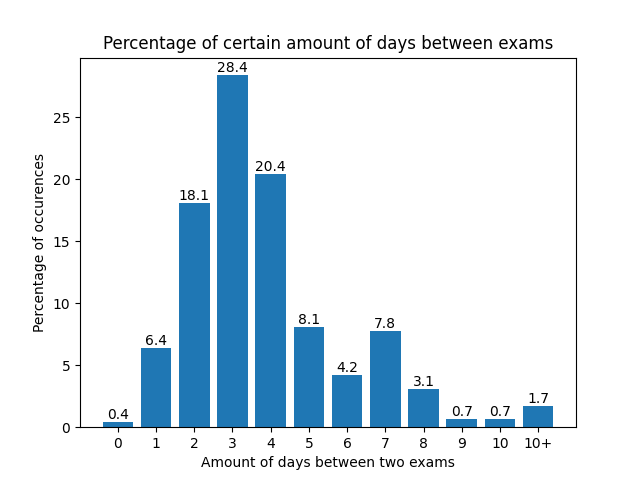
\includegraphics[width=0.5\textwidth]{images/manual/fti_sem1_percentages_manual.png}}
  \hfill
  \subfloat[FWET]{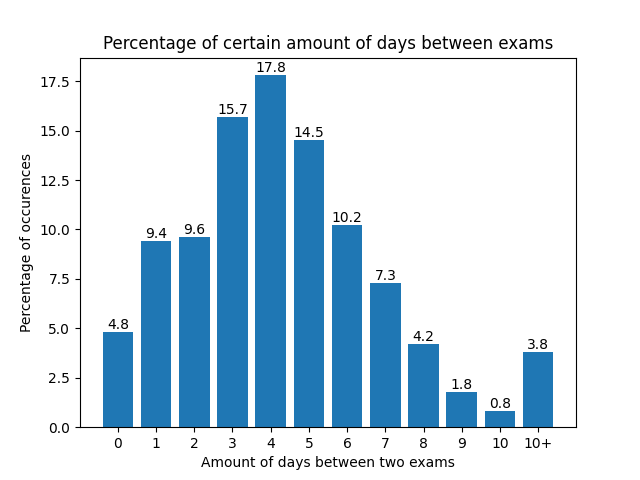
\includegraphics[width=0.5\textwidth]{images/manual/fwet_sem1_percentages_manual.png}}
  \caption{Manual exam distribution for January 2021}
  \label{fig:manual_sem1}
\end{figure}

\begin{figure}[H]
  \centering
  \subfloat[FTI]{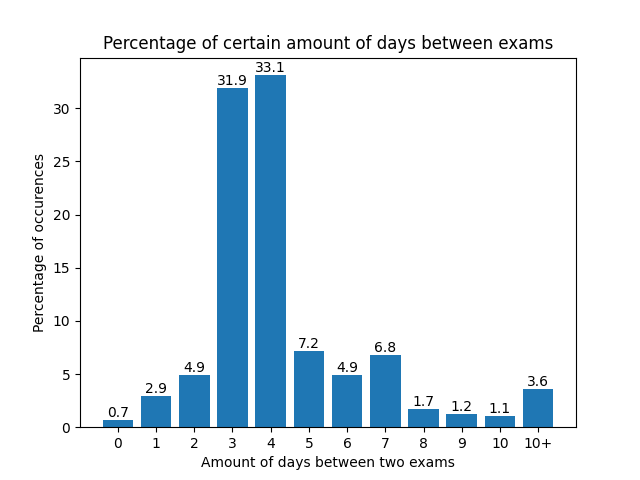
\includegraphics[width=0.5\textwidth]{images/manual/fti_sem2_percentages_manual.png}}
  \hfill
  \subfloat[FWET]{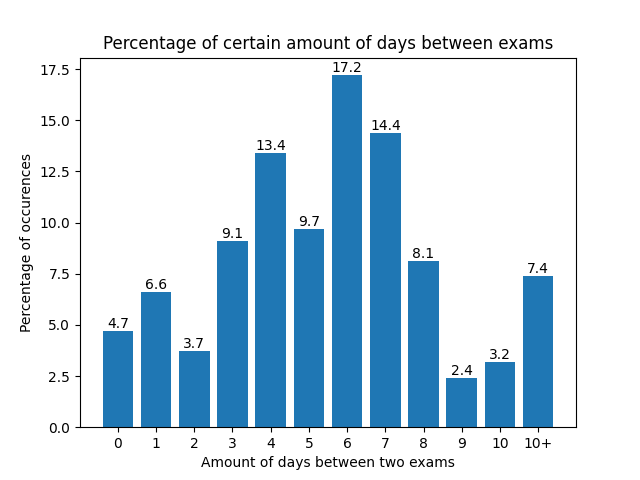
\includegraphics[width=0.5\textwidth]{images/manual/fwet_sem2_percentages_manual.png}}
  \caption{Manual exam distribution for June 2021}
  \label{fig:manual_sem2}
\end{figure}

\begin{figure}[H]
  \centering
  \subfloat[January 2021]{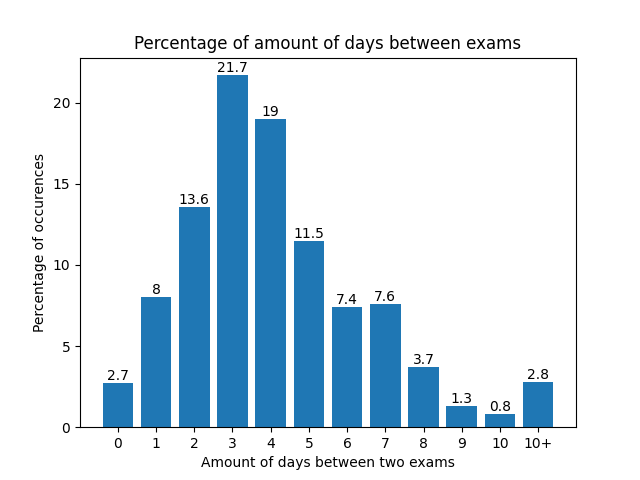
\includegraphics[width=0.5\textwidth]{images/manual/existing_combined_sem1_percentages.png}}
  \hfill
  \subfloat[June 2021]{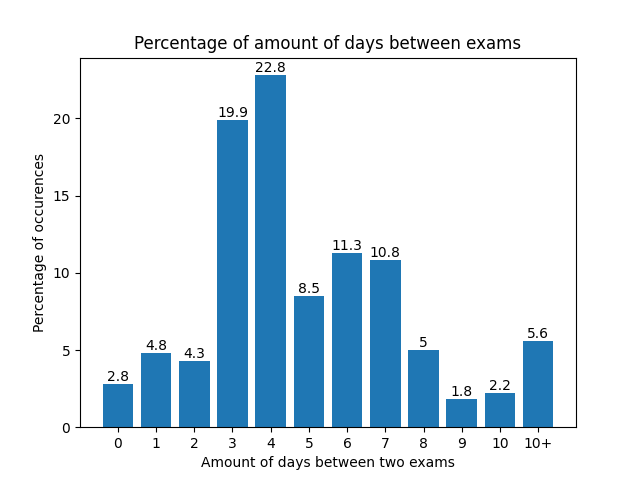
\includegraphics[width=0.5\textwidth]{images/manual/existing_combined_sem2_percentages.png}}
  \caption{Manual exam distribution for FTI and FWET combined}
  \label{fig:manual_combined}
\end{figure}


\subsection{Initialisation phase} \label{phase_init}

In order to quantify the feasibility of a solution, it is possible to look at either the objective function or the amount of hard constraint violations. Since the objective function was adapted to contain exponents and the conflict weight having a large impact on the size of the objective, looking at the amount of hard constraint violations can provide a better perspective. By plotting the violations per iteration, the progress made by the initialisation phase can be visualised. Figure \ref{fig:violations} shows the amount of exam conflicts for students. The exam conflicts are guaranteed to be the only hard constraint violations present because of how the initialisation phase generates the initial solution. There, exams are only assigned to time slots and rooms if they do not violate constraint 2, 3, and 4. This means that the room capacity, type, and availability to faculty is already taken into account. Because of this, the amount of conflicts shown is the amount of constraint 5 violations, namely the amount of times a student has multiple exams on the same day. Since the amount of conflicts reduces to 0, it proves that the initialisation phase is able to generate a solution for the Faculty of Applied Engineering and the Faculty of Science without hard constraint violations. 

It shows that the initialisation phase is able to reach a feasible solution for both data sets. Both the amount of conflicts and the execution time is higher for the January data set compared to the results for June. This can be explained by the higher workload per student for January combined with the lower amount of periods (Section \ref{sec:experiment}). This makes the amount of hard constraint violations during the initialisation solution higher, which thus requires more iterations to resolve.

\begin{figure}[H]
  \centering
  \subfloat[January 2021]{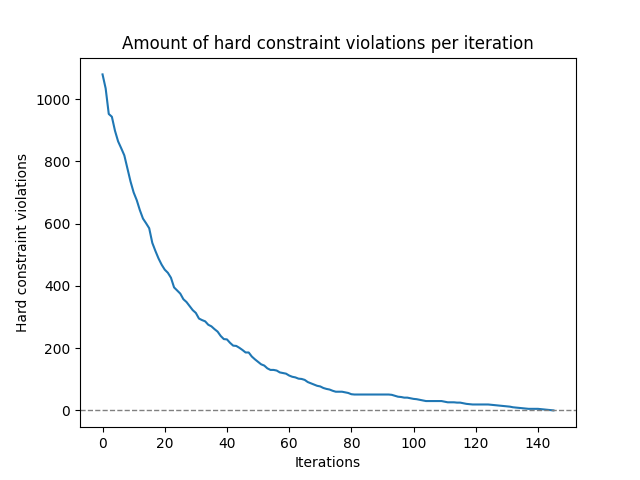
\includegraphics[width=0.5\textwidth]{images/init/sem_1_conflicts.png}}
  \hfill
  \subfloat[June 2021]{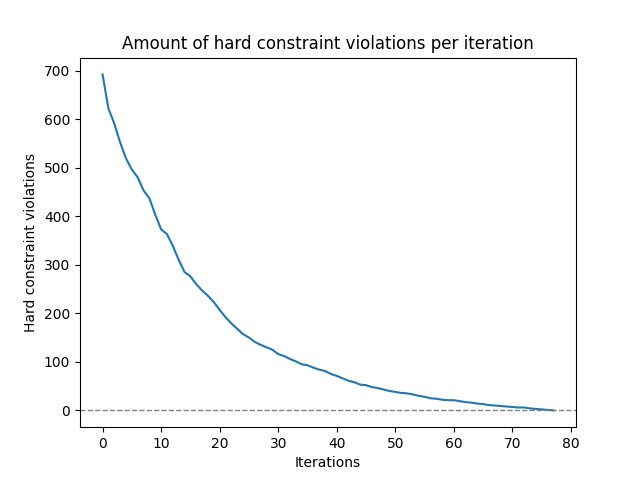
\includegraphics[width=0.5\textwidth]{images/init/sem_2_conflicts.png}}
  \caption{Hard constraint violations during initialisation phase}
  \label{fig:violations}
\end{figure}

Figure \ref{fig:phase_comparison} displays the execution time of the initialisation phase compared to the optimisation phase for the same amount of iterations. It shows that the initialisation phase is highly effective at finding a feasible solution, taking significantly less time compared to running the optimisation phase.

 
\begin{figure}[H]
  \centering
  \subfloat[January 2021]{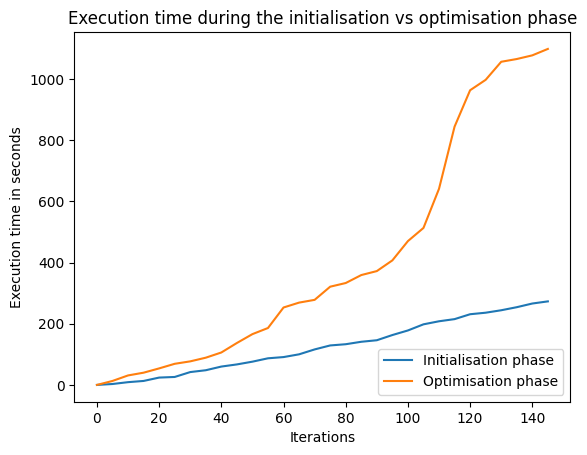
\includegraphics[width=0.5\textwidth]{images/init/sem1_phase_comparison.png}}
  \hfill
  \subfloat[June 2021]{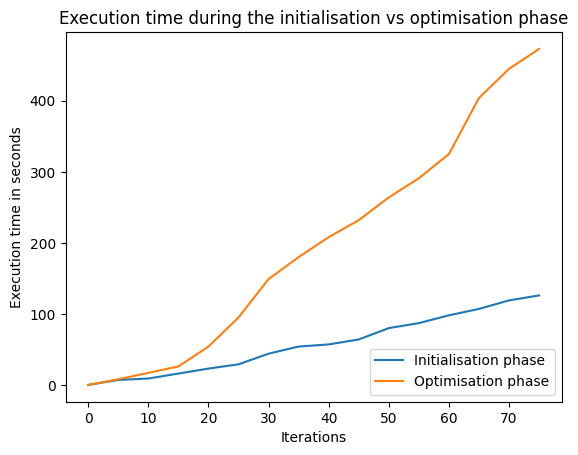
\includegraphics[width=0.5\textwidth]{images/init/sem2_phase_comparison.png}}
  \caption{Execution time comparison between initialisation and optimisation phase}
  \label{fig:phase_comparison}
\end{figure}

However, Figure \ref{fig:init} shows that no attention was given to the distribution. This can be deduced by the presence of a high percentage of exams after a single day. The exam distribution also confirms that there are no overlapping exams present after the initialisation phase.

\begin{figure}[H]
  \centering
  \subfloat[January 2021]{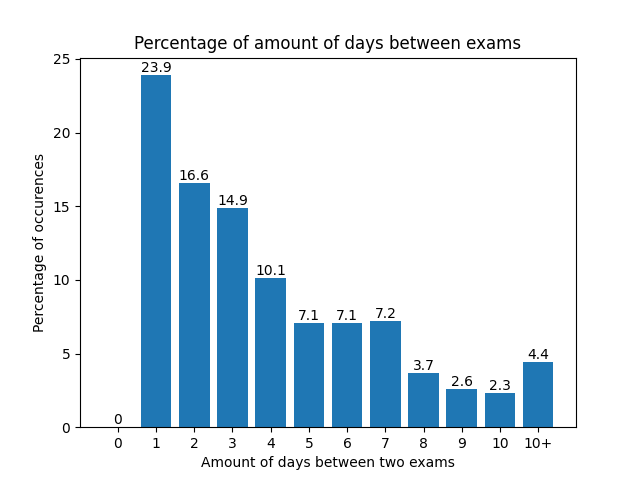
\includegraphics[width=0.5\textwidth]{images/init/sem1.png}}
  \hfill
  \subfloat[June 2021]{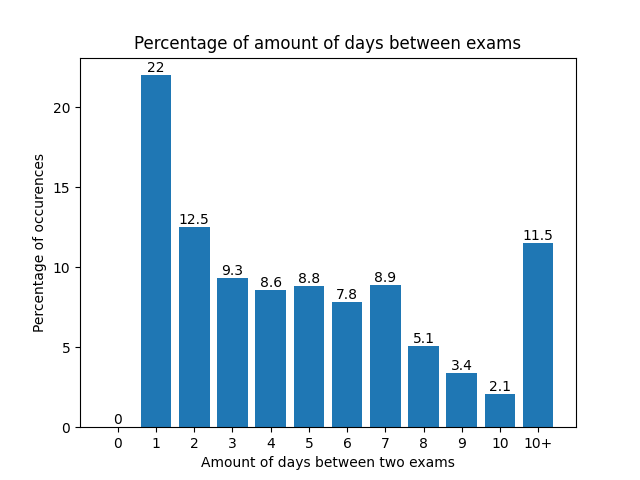
\includegraphics[width=0.5\textwidth]{images/init/sem2.png}}
  \caption{Exam distribution after the initialisation phase}
  \label{fig:init}
\end{figure}

\subsection{Optimisation phase}

While we have shown that tabu search can efficiently generate a feasible solution from the provided data set, the exam distribution will determine whether the automated schedules are superior in quality compared to the manual timetables provided by the university's administration.

First, we look at which Tabu Search version is able to generate the best results. Afterwards, we'll compare the generated timetables with the reference solutions.

\subsubsection{Comparison between Tabu Search versions}

In order to compare the different versions as explained in Section \ref{sec:method}, we look at the execution time and exam distribution.  Figure \ref{fig:version_comparison} shows the execution time when running the search algorithm versions for the two exam periods. For version 1, it shows that the execution time per iteration remains constant and is significantly lower compared to both version 2 and 3. Additionally, it can be seen that version 2 is faster than version 3. However, the difference between them depends on the data set used. This difference between version 1 and the other two versions can be explained by the change in what describes a tabu move. Instead of considering a move to be a combination of the exam and period as used in version 1, version 2 and 3 identify a move solely by the exam. Because of this change, a lot of moves that were considered not tabu in version 1 because of a different period targeted, are seen as tabu in the other versions. This makes that these versions often have to check significantly more moves, resulting in a longer execution time. This can also explain why version 2 and 3 have a similar execution time for the June data set. Whenever the search is converging, it can become difficult to find a solution that is considered superior to the one already known. This makes that the search will have to consider a high amount of moves before finding a move, that can be successfully applied. Because of this, the number of moves explored during the search in version 2 can be similar to the number explored in version 3. This is especially true when setting a smaller MAX\_MOVES parameter. 

\begin{figure}[H]
  \centering
  \subfloat[January 2021]{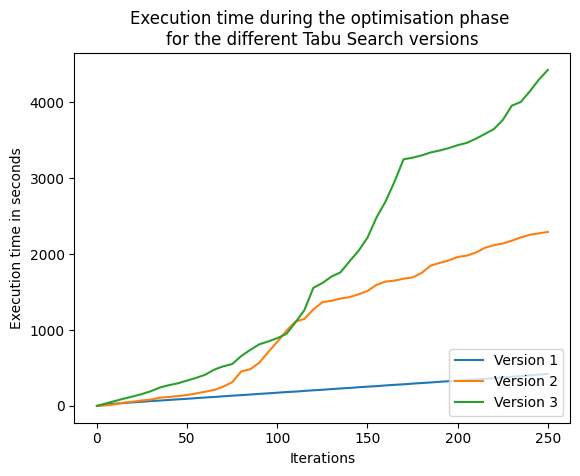
\includegraphics[width=0.5\textwidth]{images/results/versions/sem1_execution_times.png}}
  \hfill
  \subfloat[June 2021]{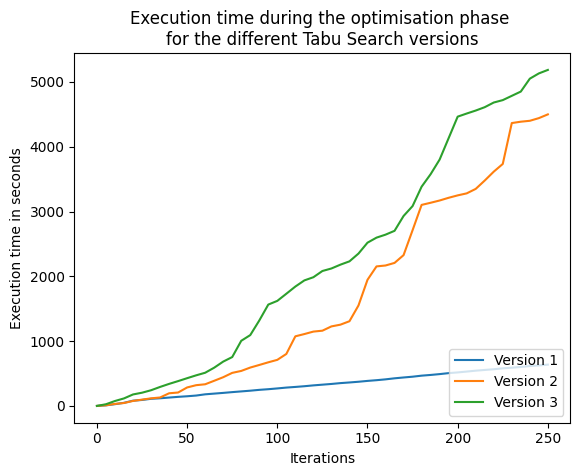
\includegraphics[width=0.5\textwidth]{images/results/versions/sem2_execution_times.png}}
  \caption{Execution time comparison between the different Tabu Search versions}
  \label{fig:version_comparison}
\end{figure}


Tables \ref{tab:version_comparison_sem1} and \ref{tab:version_comparison_sem2} detail the exam distribution after consolidating the best results from multiple runs for each version. Several conclusions can be made from these results. First, version 1 clearly performs worse compared to the other version for both data sets. This can especially be seen for the June data set where 23.9\% of the time, a student has two or fewer days between exams. This is only 15.2\% and 16.3\% for version 2 and version 3, respectively. Second, the difference in performance between version 2 and 3 is minimal. Version 2 performing equally well or better than version 3 can again be explained by the MAX\_MOVES parameter losing its importance during long runs. The reason behind this is due to the tabu move definition, which also affected the execution time. This means that we will focus on the results by version 2 in future analyses.

Finally, the difference in quality between January and June is quite notable. For January, the best result with version 2 has two or fewer days between exams 27.9\%. This is significantly worse than the best result for June, where that only occurs 15.3\% of the time.

\begin{table}[h]
	\caption{Exam distribution comparison between the different Tabu Search versions for January 2021}
	\label{tab:version_comparison_sem1}
	\centering
	\begin{tabular}{c c c c c c}
		\hline
  	\textbf{Version}	&
   \textbf{0 days \% } &
    \textbf{1 day \% } & 
    \textbf{2 days \% } &
    \textbf{3 days \% } & 
    \textbf{4+ days \%}\\ \hline
    Version 1 & 1.9\% & 16.7\% & 14.7\% & 18.4\% & 48.3\% \\
    Version 2 & 0.1\% & 14.5\% & 13.3\% & 20.6\% & 51.5\% \\
    Version 3 & 0.1\% & 15.3\% & 13.1\% & 24.6\% & 46.9\% \\
        \hline
	\end{tabular}
\end{table}

\begin{table}[h]
	\caption{Exam distribution comparison between the different Tabu Search versions for June 2021}
	\label{tab:version_comparison_sem2}
	\centering
	\begin{tabular}{c c c c c c}
		\hline
  	\textbf{Version}	&
   \textbf{0 days \% } &
    \textbf{1 day \% } & 
    \textbf{2 days \% } &
    \textbf{3 days \% } & 
    \textbf{4+ days \%}\\ \hline
    Version 1 & 0.2\% & 11.5\% & 12.2\% & 17.2\% & 58.9\% \\
    Version 2 & 0.0\% & 6.8\% & 8.4\% & 24.3\% & 60.5\% \\
    Version 3 & 0.3\% & 7.8\% & 8.2\% & 22.0\% & 61.7\% \\
        \hline
	\end{tabular}
\end{table}
 \label{subsec:versions}
\subsubsection{Comparison between generated and reference solutions}

The results from Section \ref{subsec:versions} allow us to determine the best version and with it the best generated solution. However, we must compare the generated solutions with the reference solutions in order to answer the question whether the automated solutions outperform the manual timetables. Figures \ref{fig:sem1_comparison} and \ref{fig:sem2_comparison} provide the exam distribution of the generated solutions next to the reference solutions. 

The generated solution for January 2021 has two or fewer days between exams 27.9\% of time, while that is only 12\% for the reference solution.  Although a smaller difference, the same can be observed for June with a percentage of 15.4\% and 11.9\% for the generated and reference solution, respectively. However, the distribution looks very different with the generated solutions having nearly no exam conflicts. This does occur for the reference solution, for almost 3\% of the time in the solutions for both data sets.


\begin{figure}[H]
  \centering
  \subfloat[Reference solution]{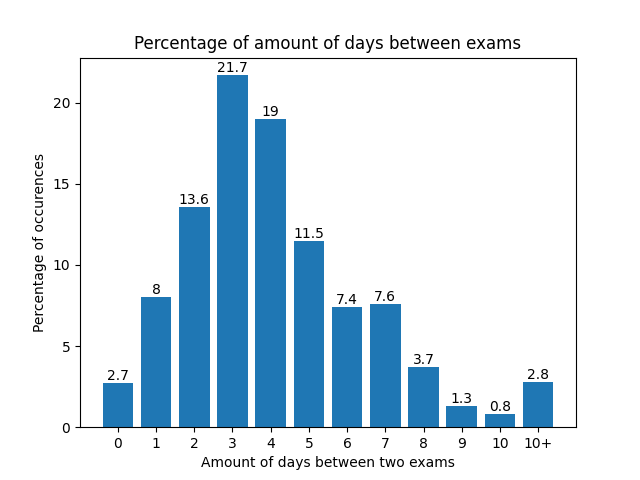
\includegraphics[width=0.5\textwidth]{images/manual/existing_combined_sem1_percentages.png}}
  \hfill
  \subfloat[Generated solution]{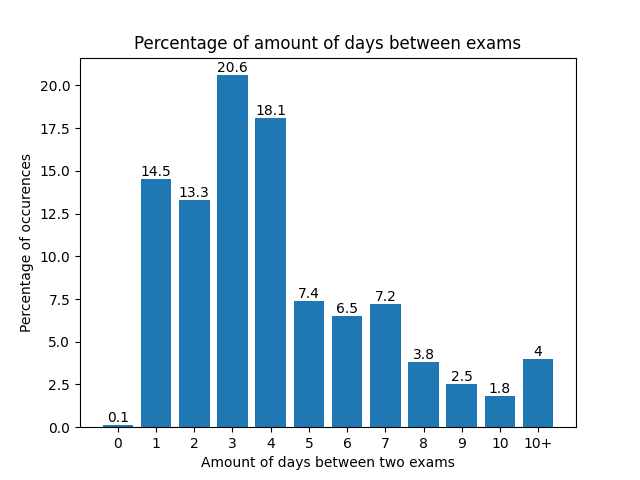
\includegraphics[width=0.5\textwidth]{images/results/final/sem1_generated.png}}
  \caption{Exam distribution comparison for January 2021}
  \label{fig:sem1_comparison}
\end{figure}

\begin{figure}[H]
  \centering
  \subfloat[Reference solution]{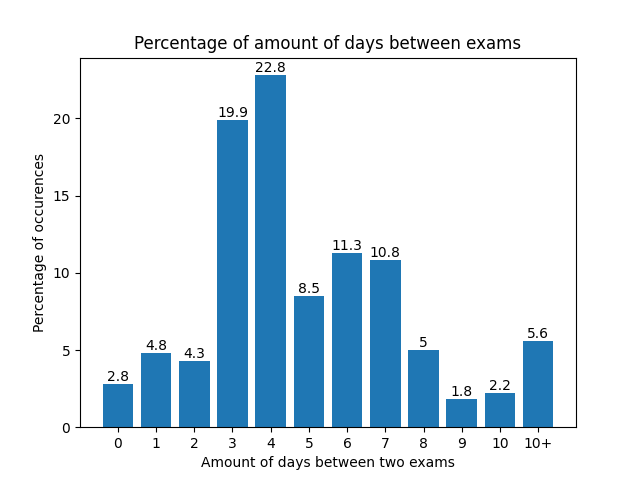
\includegraphics[width=0.5\textwidth]{images/manual/existing_combined_sem2_percentages.png}}
  \hfill
  \subfloat[Generated solution]{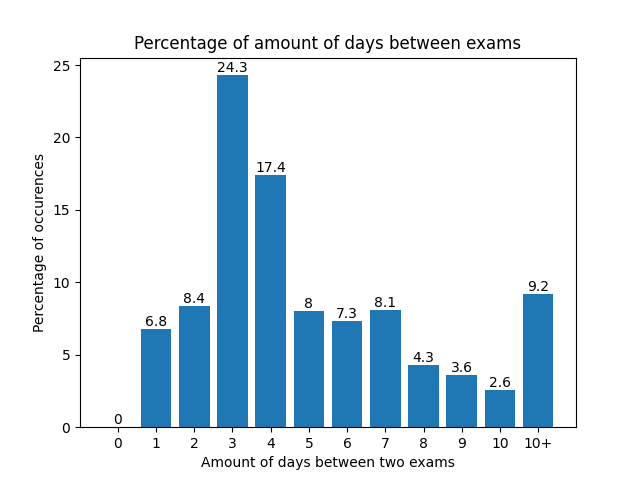
\includegraphics[width=0.5\textwidth]{images/results/final/sem2_generated.png}}
  \caption{Exam distribution comparison for June 2021}
  \label{fig:sem2_comparison}
\end{figure}

\subsubsection{Qualitative feedback on the generated solutions}

In addition to the quantitative comparison between the generated and reference solutions, we also reviewed the obtained timetables with the university administrators. This was done by providing them with the timetables in Excel format, as detailed in Section \ref{qualitative}, and with the exam distribution figures visible in Figures 
\ref{fig:generated_sem1} and \ref{fig:generated_sem2}. These figures provide a more detailed view on the exam distribution by splitting the two faculties. 

\begin{figure}[H]
  \centering
  \subfloat[Faculty of Applied Engineering]{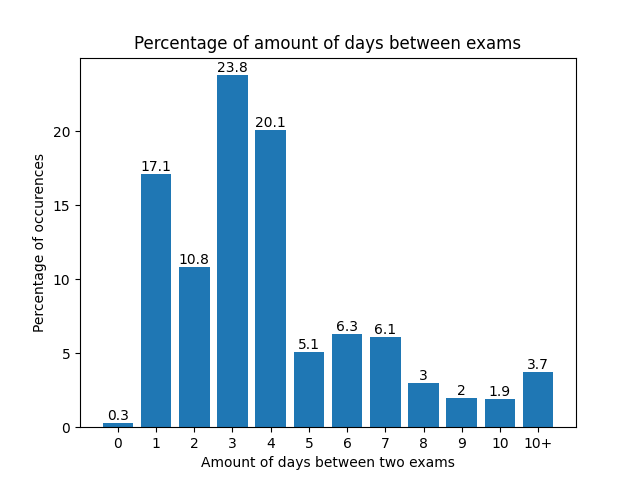
\includegraphics[width=0.5\textwidth]{images/results/final/fti_sem1.png}}
  \hfill
  \subfloat[Faculty of Science]{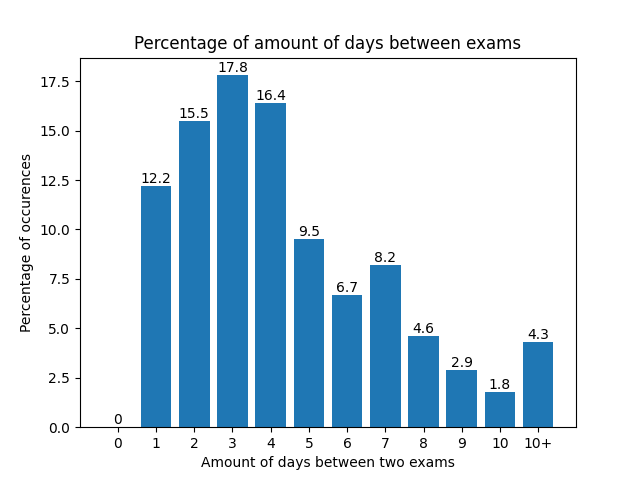
\includegraphics[width=0.5\textwidth]{images/results/final/fwet_sem1.png}}
  \caption{Generated exam distribution for January 2021}
  \label{fig:generated_sem1}
\end{figure}

\begin{figure}[H]
  \centering
  \subfloat[Faculty of Applied Engineering]{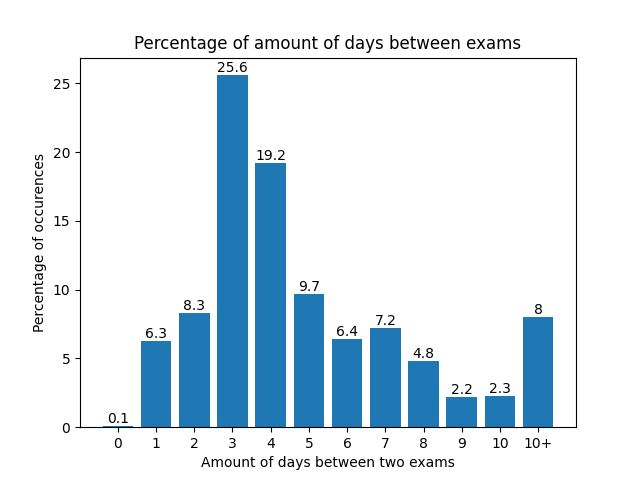
\includegraphics[width=0.5\textwidth]{images/results/final/fti_sem2.png}}
  \hfill
  \subfloat[Faculty of Science]{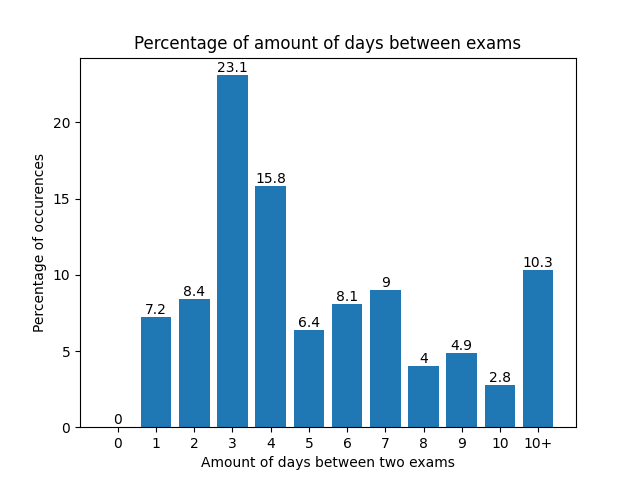
\includegraphics[width=0.5\textwidth]{images/results/final/fwet_sem2.png}}
  \caption{Generated exam distribution for June 2021}
  \label{fig:generated_sem2}
\end{figure}

They were able to add insights that are not visible in the quantitative results. First, they note that the search method correctly takes into account exams that belong to different enrolment years within the model track. For example, some of the students that have two exams scheduled on consecutive days, only have this for exams that are not part of the same year. While this negatively impacts the distribution statistics, its actual impact is minimal because no priority is given to two exams that are not within the same year for the model track. However, the model track has no extra weight when assigning exams to time slots, resulting in cases where a model track student only has a single day between exams. The university's administration strongly attempts to prevent this, often at the cost of the distribution for non-model track students. The presence of these cases reduces the feasibility of using the generated solutions.

Second, they confirm that the search algorithm prioritises exams with a large amount of students enrolled over small exams. Since we consider all students that are enrolled for every exam, the penalties incurred by poorly scheduled large exams have a significant impact on the objective function. 

Finally, they conclude that while the obtained distribution is not currently sufficient as final solution, the generated solutions can act as an initial baseline. This would reduce the time spent on generating an initial solution. The solution could then be further optimised manually.


